\newpage
МРНТИ 52.47.27
\hfill {\bfseries \href{https://doi.org/10.58805/kazutb.v.3.24-513}{https://doi.org/10.58805/kazutb.v.3.24-513}}

\sectionwithauthors{Т.С. Кайненова, Г.Т. Космбаева, А.Т. Отарбаева, А. Мерекеқызы}{АНАЛИЗ СОСТОЯНИЯ ВЫРАБОТКИ ЗАПАСОВ НЕФТИ ИЗ ПЛАСТОВ НА МЕСТОРОЖДЕНИИ СЕВЕРНАЯ ТРУВА}

\begin{center}
Т.С. Кайненова\envelope, Г.Т. Космбаева, А.Т. Отарбаева, А.
Мерекеқызы

Актюбинский региональный университет им.К. Жубанова, Актобе, Казахстан,
\end{center}
\envelope Корреспондет-автор: kaynenova83@mail.ru


Эффективность систем разработки нефтяных месторождений во многом
определяется всеми возможными методами разработки промышленных нефтяных
запасов, характером добычи. Рост темпов производства, высокий спрос на
нефтепродукты, требуют полного извлечения нефти из недр. Основной целью
исследования является анализ состояния добычи запасов нефти на
месторождении Северная Трува путем выявления проблем, возникающих при
добыче запасов нефти в продуктивных пластах, повышения интенсивности
добычи нефти, анализа результатов теоретических и экспериментальных
исследований. При разведке и исследовании запасов нефти и газа важна
производительность слоя, поскольку физическая среда слоя изменяется с
каждой полученной молекулой в процессе добычи, чем дольше слой работает,
тем точнее прогноз остальных запасов. В ходе исследования изучаются
особенности геологического строения нефтяных месторождений, изучается
влияние на гидродинамические процессы в них, проводится работа по
обоснованию геологических и профессиональных критериев, определяющих
эффективное развитие.

В статье изучается метод совершенствования методов оценки
эксплуатационных параметров и обоснования конструктивных особенностей
завершения при вскрытии капитально построенных месторождений.
Предусматривается увеличение добычи нефтяных запасов капитально
построенных месторождений путем обоснования технологических параметров
эксплуатации скважин.

Ключевые слова: Запас нефти, пласт, скважина, дебит нефти, газовый
фактор, фонтанирование, механизирование.

\sectionheading{СОЛТҮСТІК ТРУВА КЕН ОРНЫНДАҒЫ ҚАБАТТАРДАН МҰНАЙ ҚОРЛАРЫН ӨНДІРУ ЖАҒДАЙЫН ТАЛДАУ}

\begin{center}
{\bfseries Т.С. Кайненова\envelope, Г.Т. Космбаева, А.Т.
Отарбаева, А. Мерекеқызы}

Қ. Жұбанов атындағы Ақтөбе өңірлік университеті, Ақтөбе, Қазақстан,

е-mail: kaynenova83@mail.ru
\end{center}

Мұнай кен орындарын игеру жүйелерінің тиімділігі көбінесе өнеркәсіптік
мұнай қорларын игерудің барлық мүмкін әдістерімен, өндіріс сипатымен
анықталады. Өндіріс қарқынының өсуі, мұнай өнімдеріне жоғары сұраныс жер
қойнауынан мұнайды толық алуды талап етеді. Зерттеудің негізгі мақсаты
өнімді қабаттардағы мұнай қорларын өндіру кезінде туындайтын
проблемаларды анықтау, мұнай өндіру қарқындылығын арттыру, теориялық
және эксперименттік зерттеулердің нәтижелерін талдау арқылы Солтүстік
Трува кен орнындағы мұнай қорларын өндіру жағдайын талдау болып
табылады. Мұнай мен газ қорларын барлау және зерттеу кезінде қабаттың
өнімділігі маңызды, өйткені қабаттың физикалық ортасы өндіру процесінде
алынған әрбір молекуламен өзгереді, қабат неғұрлым ұзақ жұмыс істесе,
қалған қорлардың болжамы соғұрлым дәл болады. Зерттеу барысында мұнай
кен орындарының геологиялық құрылымының ерекшеліктері зерттеледі,
олардағы гидродинамикалық процестерге әсері зерттеледі, тиімді дамуды
анықтайтын геологиялық және кәсіби критерийлерді негіздеу бойынша жұмыс
жүргізіледі.

Мақалада күрделі салынған кен орындарын ашу кезінде пайдалану
параметрлерін бағалау әдістерін жетілдіру және аяқталудың құрылымдық
ерекшеліктерін негіздеу әдісі зерттеледі. Ұңғымаларды пайдаланудың
технологиялық параметрлерін негіздеу арқылы күрделі салынған кен
орындарының мұнай қорларын өндіруді ұлғайту көзделеді.

Түйін сөздер: мұнай қоры, қабат, ұңғыма, мұнай дебиті, газ факторы,
фонтандау, механикаландырылған.

\sectionheading{ANALYSIS OF THE STATE OF PRODUCTION OF OIL RESERVES FROM RESERVOIRS AT THE NORTH TRUVA FIELD}

\begin{center}
{\bfseries T.S. Kainenova\envelope, G.T. Kosmbayeva, A.T.
Otarbayeva, A. Merekeqyzy}

Aktobe Regional University named after K. Zhubanov, Aktobe, Kazakhstan,

е-mail: kaynenova83@mail.ru
\end{center}

The effectiveness of oil field development systems is largely determined
by all possible methods of developing industrial oil reserves and the
nature of production. The growth of production rates, high demand for
petroleum products, require the complete extraction of oil from the
subsoil. The main purpose of the study is to analyze the state of oil
reserves production at the Severnaya Truva field by identifying problems
that arise during the extraction of oil reserves in productive
formations, increasing the intensity of oil production, analyzing the
results of theoretical and experimental studies. In the exploration and
exploration of oil and gas reserves, the productivity of the layer is
important, since the physical environment of the layer changes with each
molecule obtained during the extraction process, the longer the layer
works, the more accurate the forecast of the remaining reserves. In the
course of the study, the features of the geological structure of oil
fields are studied, the influence on hydrodynamic processes in them is
studied, work is being carried out to substantiate geological and
professional criteria that determine effective development.

The article examines the method of improving the methods of evaluating
operational parameters and substantiating the design features of
completion during the opening of capital-built deposits. It is envisaged
to increase the production of oil reserves of capital-built fields by
substantiating the technological parameters of well operation.

Keywords: Oil reserve, reservoir, well, oil flow rate, gas factor,
gushing, mechanization.

\begin{multicols}{2}
{\bfseries Введение.} Актуальность темы исследования "Анализ состояния выработки
запасов нефти из пластов на месторождении Северная Трува" обусловлена
несколькими ключевыми аспектами. Во-первых, развитие современных
нефтяных месторождений требует полного извлечения нефти из недр, что
является актуальной задачей в условиях роста потребления и высокой
востребованности нефтепродуктов на мировом рынке. Эффективность
разработки месторождений напрямую зависит от применения оптимальных
методов добычи и управления пластовыми системами, что требует глубокого
анализа текущих процессов и параметров эксплуатации.

Во-вторых, особенности геологического строения и гидродинамических
процессов в пластах месторождения Северная Трува требуют точного
прогноза оставшихся запасов нефти и выбора эффективных технологических
решений для максимизации коэффициента извлечения. Исследование
направлено на выявление и устранение проблем, возникающих в ходе
эксплуатации скважин, что способствует повышению интенсивности добычи и
более рациональному использованию ресурсов.

Таким образом, тема исследования имеет высокую практическую значимость,
так как результаты анализа могут быть использованы для улучшения методов
разработки нефтяных месторождений, повышения производительности и
устойчивости нефтедобычи в долгосрочной перспективе {[}1,2{]}.

Научная новизна исследования заключается в проведении детального анализа
состояния разработки нефтяных запасов на месторождении Северная Трува с
акцентом на геологические и гидродинамические особенности пластов, что
позволяет выявить ключевые проблемы и предложить способы их решения.
Исследование направлено на усовершенствование методов оценки
эксплуатационных параметров и обоснование конструктивных решений для
повышения эффективности извлечения нефти. Новизна также заключается в
разработке рекомендаций по интенсификации добычи нефти, учитывая
особенности эксплуатации скважин и изменения физических свойств пластов
в процессе их разработки, что ранее не получало достаточного внимания.
Предложенные методы позволяют оптимизировать работу существующих и новых
скважин, а также улучшить управление газовым фактором и водоотбором, что
способствует более полному извлечению углеводородов из недр.

Модель месторождения Северная Трува основывалась на результатах
интерпретации трехмерных сейсмических материалов, отобранных Даганским
филиалом института при геофизической компании «Восток» и данных бурения
55 скважин. По этим данным структура Северная Трува по кровле
карбонатных толщ КТ-I и КТ-II представляла собой пологую широкую
брахиантиклиналь северо-восточного простирания, ограниченную с
юго-востока региональным разломом F. Площадь структуры Северная Трува
значительно увеличивается в юго-западном и северном направлениях.
Тектоническая схема подсолевых отложений Восточной части Прикаспийской
впадины (Рисунок 1) {[}3{]}.

К основным технологическим факторам, влияющим на показатели нефтедобычи
резервуаров, относятся параметры сети добывающих скважин, основная схема
системы затопления, темпы развития, отбор нагнетательной жидкости,
технология откачки воды и условия развития прилегающих пластов, характер
вскрытия продуктивных пластов в скважинах. Исследование влияние
обводнения продуктивных слоев на полноту добычи, в зависимости от
степени охвата как по площади объекта разработки, так и с точки зрения
рубок, характера перекачиваемой воды и смещения пласта. Поэтому при
геологическом и профессиональном анализе необходимо уделять основное
внимание особенностям движения воды по продуктивным слоям под влиянием
перекачки воды. К числу геологических и физических факторов, влияющих на
процесс слоистого затопления, относятся фильтрующие свойства
продуктивных слоев, их неоднородные свойства и степень их
неоднородности, вязкостные свойства насыщенных слоев и перекачиваемых в
них жидкостей {[}4,5{]}.

{\bfseries Материалы и методы}. Нефтяные запасы можно оценить по динамике
интенсивности добычи, коэффициенту текущей подачи нефти и количеству
перекачиваемой воды. Темпы отбора нефти и текущая нефтеотдача
анализируются в динамике по годам развития производства и дате анализа.
Эти показатели определяются для месторождений в целом и для отдельных
районов, блоков, участков и пластов разработки в зависимости от их
первоначальных балансовых запасов {[}6{]}.

Добыча нефтяных запасов также характеризуется темпами добычи нефти из
первичных извлекаемых запасов нефти и текущей передачей нефти.
Балансовые запасы нефти часто используются при попытке избежать ошибок в
определении запасов нефти, а также при сравнительном анализе с другими
месторождениями.

Месторождение Северная Трува в административном отношении расположено на
территории Муголжарского района Актюбинской области Республики
Казахстан.

Нефтегазоносность месторождения связана с отложениями двух карбонатных
толщ. Продуктивные пласты месторождения Северная трува приурочены к
средне-нижнему карбону регионально - нефтегазоносному комплексу пород,
представленному двумя мощными толщами карбонатов (КТ-I и КТ-II),
сложенных из известняка и доломитов {[}7{]}.
\end{multicols}

\begin{figure}[H]
	\centering
	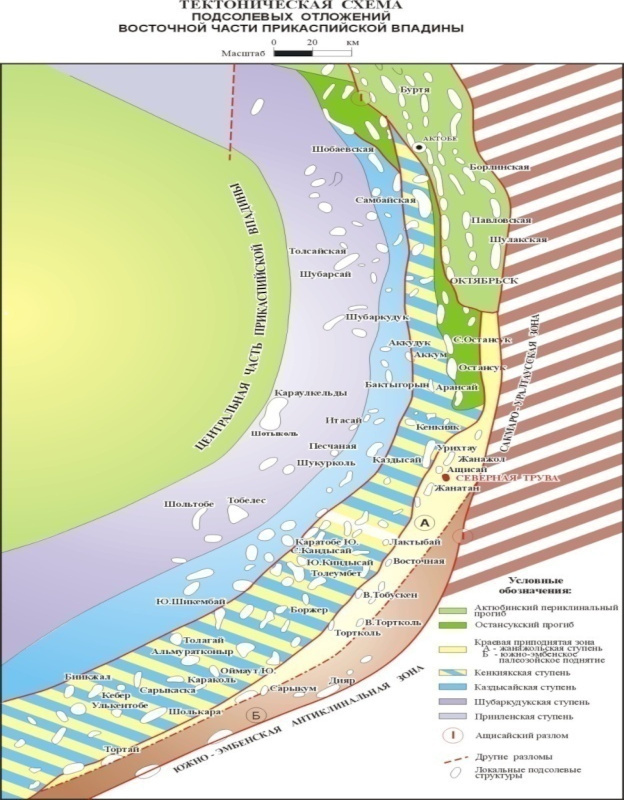
\includegraphics[width=0.8\textwidth]{assets/301}
	\caption*{Рис. 1 - Тектоническая схема подсолевых отложений Восточной
части Прикаспийской впадины}
\end{figure}

\begin{multicols}{2}
В эксплуатационном фонде месторождения Северная Трува добывающих скважин
находятся 164 ед., в том числе 150 действующих, 12 в бездействии, 1 ед.
в освоении и 1 ед. в ожидании освоения после бурения. Скважины
добывающего фонда эксплуатируются механизированным и фонтанным
способами.

С последнего проектного документа «Дополнение к технологической схеме
разработки\ldots» (2015г) на месторождении введены из бурения 38 новых
скважин, из них 3 оценочные скважины, 1 скважина находится в освоении
после бурения, 1 скважина в ожидании освоения:

\begin{itemize}
\item
  Пачка А -- 7 скважин;
\item
  Пачки А+Б -- 3 скважин;
\item
  Пачка Гв-- 10 скважин;
\item
  Пачки Гв+Гн-- 6 скважин;
\item
  Пачка Гн -- 7 скважин.
\end{itemize}

\emph{I объект КТ-1 (А+Б)}

В эксплуатационном фонде добывающих скважин числятся 101ед, а т.ч.
действующие 90, в бездействии 11 скважин. Все скважины кроме скважин
№СТ-24, 484, которые эксплуатируются УЭЦН, работают фонтанным способом
эксплуатации. В освоении после бурения находится одна скважина. 6
скважин эксплуатируются совместно на пачках А+Б.

\emph{II объект -- КТ-2 (Гв+Гн)}

Фонд добывающих скважин составил 63 ед., из них 60 ед. действующие,
скважина №5597 числится в бездействии, скважина №8106 находится в
освоении после бурения и скважина №5633 в ожидании освоения. Также 5
скважин находятся в консервации.

В целом добывающий фонд эксплуатируется фонтанным и механизированным
способами. 59 скважин работают фонтанным способом, 1 скважина (№7615)
газлифтным и 2 скважины (№№7674,7708) НДГ. В целом скважины размещены
равномерно по пачкам.

За отчетный период из бурения в эксплуатацию введено 22 добывающих (1
находится в освоении после бурения, 1 в ожидании освоения после бурения)
и 3 нагнетательных скважин (№№5575, 5617, 5623). Одна добывающая
скважина (СТ-15) была переведена с Iобъекта. 34 добывающих скважин были
переведены в нагнетательный фонд. Стоит заметить, что фонд
нагнетательных скважин увеличился в основном за счёт перевода скважин из
добывающего фонда {[}2,3{]}.

{\bfseries Результаты и обсуждение.} Для оценки эффективности реализуемой
системы разработки месторождения и выработки на этой основе рекомендаций
по совершенствованию системы разработки проведен анализ основных
технологических показателей работы скважин {[}8{]}.

Нефтяная группа определялась на основе трех параметров - воды, хлористых
солей и механических примесей в пробах.

По средним значениям, нефти толщ КТ-I и КТ-II классифицируются как
малосернистые и сернистые и принадлежат первому и второму классам. По
среднему значению нефть толщи KT-I относится к третьей группе: с
содержанием хлористых солей -- 209.2 мг/дм\textsuperscript{3}, - воды --
1.04 мас.\%, - механических примесей не выше нормы. Нефти толщи КТ-II
условно относятся к третьей группе: с содержанием хлористых солей --
641.7 мг/дм\textsuperscript{3}, - воды -- 2.00 мас.\% (выше нормы) -
механических примесей в норме. При этом в общей массе анализов
фиксируются пробы, принадлежащие к первой, второй и третьей группам. По
ряду проб зафиксированы аномальные содержания солей (до 3426
мг/дм\textsuperscript{3}) и воды (8.8 мас.\%), которые не укладываются в
рамки стандарта классификации {[}9{]}.

Потенциал продуктивного горизонта зависит от литологического состава
породы, эффективной мощности~пласта, коллекторских свойств (объёма
порового пространства), степени~нефте-~и (или)~газонасыщения,
величины~вязкости~флюида~и термобарических условий, а также от способов
и интенсивности физико-химических методов воздействия на пласт при
разработке месторождения с целью повышения его~нефте- и
(или)~газоотдачи. Продуктивный горизонт является основным объектом
подсчёта запасов~нефти~и~газа.~На месторождении Северная Трува
пористость вычисляется путем построения кроссплотов по данным
литолого-плотностного каротажа, компенсированного нейтронного каротажа,
акустического каротажа определяется общая пористость, эффективная
пористость выделенных пластов-коллекторов {[}10{]}.

Верхняя карбонатная толща КТ-I, с которой связана
газоконденсатнонефтяная залежь, в стратиграфическом отношении приурочена
к отложениям касимовско-гжельского возраста.

Нижняя карбонатная толща КТ-II, содержащая газонефтеконденсатную залежь,
приурочена к отложениям верейско-каширского возраста. Коллекторские и
физико-химические свойства продуктивных горизонтов указано в таблицах 1
и 2 {[}11{]}.
\end{multicols}

\begin{table}[H]
\caption*{Таблица 1- Физико-химическая характеристика нефти}
\centering
\begin{tabular}{|l|l|l|l|}
\hline
Объект & Содержание серы & Плотность нефти & \begin{tabular}[c]{@{}l@{}}Содержание\\   парафинов\end{tabular} \\ \hline
КТ-I & до 0,88\% & от 807,0 до 849,0 кг/м3 & от 1,67 до 5,20 \% \\ \hline
КТ-II & от 0,01 до 1,46\% & от 801,1 до 899,0 кг/м3 & от 1,93 до 4,10 \% \\ \hline
\end{tabular}
\end{table}

\begin{table}[H]
\caption*{Таблица 2- Коллекторские свойства продуктивных горизонтов}
\centering
\begin{tabular}{|l|p{0.12\textwidth}|p{0.3\textwidth}|p{0.16\textwidth}|p{0.08\textwidth}|p{0.1\textwidth}|}
\hline
Объект & Абсолютная глубина & Породы & Общая средняя толщина пласта & Порис-тость & Проницае-мость \\ \hline
КТ-I & 2095 – 2510м & известняки, доломиты, с прослойками терригенных, преимущественно аргиллитовых пород & 466м & 15,19\% & 34,02 мД \\ \hline
КТ-II & 2843 – 3021м & известняки с прослоями зеленовато-серых аргиллитов и доломитов & 320м & 12\% & 56,6 мД \\ \hline
\end{tabular}
\end{table}

\begin{table}[H]
\caption*{Таблица 3- Динамика распределения действующего фонда по дебитам нефти по объектам на 01.01.2022 г}
\centering
\begin{tabular}{|lll|l|l|l|}
\hline
\multicolumn{3}{|l|}{Объект} & КТ-1 & КТ-2 & Месторождение \\ \hline
\multicolumn{3}{|l|}{Фонд скважин} & 90 & 60 & 150 \\ \hline
\multicolumn{3}{|l|}{Средний дебит нефти} & 8,6 & 20,9 & 13,5 \\ \hline
\multicolumn{1}{|p{0.2\textwidth}|}{\multirow{10}{=}{Диапазон изменения дебитов нефти, т/сут}} & \multicolumn{1}{l|}{\multirow{2}{*}{q≤5}} & Кол-во & 52 & 9 & 61 \\ \cline{3-6} 
\multicolumn{1}{|l|}{} & \multicolumn{1}{l|}{} & \% & 57,8 & 15 & 40,7 \\ \cline{2-6} 
\multicolumn{1}{|l|}{} & \multicolumn{1}{l|}{\multirow{2}{*}{5<q≤10}} & Кол-во & 12 & 6 & 18 \\ \cline{3-6} 
\multicolumn{1}{|l|}{} & \multicolumn{1}{l|}{} & \% & 13,3 & 10 & 12 \\ \cline{2-6} 
\multicolumn{1}{|l|}{} & \multicolumn{1}{l|}{\multirow{2}{*}{10<q≤25}} & Кол-во & 17 & 23 & 40 \\ \cline{3-6} 
\multicolumn{1}{|l|}{} & \multicolumn{1}{l|}{} & \% & 18,9 & 38,3 & 26,7 \\ \cline{2-6} 
\multicolumn{1}{|l|}{} & \multicolumn{1}{l|}{\multirow{2}{*}{25<q≤50}} & Кол-во & 8 & 17 & 25 \\ \cline{3-6} 
\multicolumn{1}{|l|}{} & \multicolumn{1}{l|}{} & \% & 8,9 & 28,3 & 16,7 \\ \cline{2-6} 
\multicolumn{1}{|l|}{} & \multicolumn{1}{l|}{\multirow{2}{*}{50≥q}} & Кол-во & 1 & 5 & 6 \\ \cline{3-6} 
\multicolumn{1}{|l|}{} & \multicolumn{1}{l|}{} & \% & 1,1 & 8,3 & 4 \\ \hline
\end{tabular}
\end{table}

\begin{multicols}{2}
Анализ текущих среднесуточных показателей работы скважин и динамика
распределения действующего фонда по дебитам нефти показана в таблице 3.
Согласно проведенному распределению фонда добывающих скважин по дебитам
нефти большая часть скважин работает с дебитами до 5 т/сут -- 40,7\% от
действующего фонда скважин месторождения и большинство из них
эксплуатируются на I объекте, доля которых там составляет 57,2\%, тогда
как их доля на IIобъекте не превышает 15\%. Однако стоит учитывать, что
значительная часть из данных скважин работают периодически. Скважины со
средним дебитом от 10 до 25т/сут занимают 26\% всего действующего фонда.
Также к скважинам со сравнительно высоким дебитом от 25 т/сут относится
20,7\% действующего фонда, большинство из которых эксплуатируются на
IIобъекте. Остальные 12\% скважин на месторождении эксплуатируются с
дебитом от 5 до 10т/сут. Из данного распределения скважин по дебитам,
можно сделать вывод, что скважины IIобъекта характеризуются более
высокими дебитами по сравнению с I объектом {[}2,3{]}.

Интенсификация отборов нефти на месторождении сопровождается высокими
показателями газового фактора по I и II объекту, который на дату отчета
по составил 964 и 985 м\textsuperscript{3}/т объектам соответственно.

Как видно из таблицы 4 по распределению газового фактора видно, что
наибольшая часть скважин по объектам и соответственно по всему
месторождению (84\%) работают с показателями по газовому фактору от 900
до 1000 м\textsuperscript{3}/т. Со значениями газового фактора менее
900м\textsuperscript{3}/т и в диапазоне от 1000 до 1100
м\textsuperscript{3}/т эксплуатируются оставшиеся 16 \% действующего
фонда добывающих скважин месторождения.

Высокий газовый фактор по некоторым скважинам обусловлен возможным
дегазацией скважин, ак как наблюдается падения пластового давления ниже
давления насыщения. По данному фонду рекомендуется перевести скважины в
бездействия или перевести на более щадящий режим разработки, с
проведением периодических ГДИС, с целью прослеживания динамики
восстановления пластового давления. Прорыв из газовой шапки возможен,
однако перфорация скважин не охватывает интервалы насыщенности газа,
рекомендуется провести ГИС исследования по определению текущего
положения насыщения.
\end{multicols}

\begin{table}[H]
\caption*{Таблица 4 - Динамика распределения фонда скважин по газовому фактору}
\centering
\begin{tabular}{|lll|l|l|l|}
\hline
\multicolumn{3}{|l|}{Объект} & КТ-1 & КТ-2 & Месторождение \\ \hline
\multicolumn{3}{|l|}{Фонд скважин} & 90 & 60 & 150 \\ \hline
\multicolumn{3}{|l|}{Средний газовый фактор} & 964,4 & 984,9 & 972,6 \\ \hline
\multicolumn{1}{|p{0.2\textwidth}|}{\multirow{10}{=}{Диапазон изменения газового фактора, м3/т}} & \multicolumn{1}{l|}{\multirow{2}{*}{ГФ≤800}} & Кол-во & 3 & 1 & 4 \\ \cline{3-6} 
\multicolumn{1}{|l|}{} & \multicolumn{1}{l|}{} & \% & 3,3 & 1,7 & 2,7 \\ \cline{2-6} 
\multicolumn{1}{|l|}{} & \multicolumn{1}{l|}{\multirow{2}{*}{800<ГФ≤900}} & Кол-во & 11 & 1 & 12 \\ \cline{3-6} 
\multicolumn{1}{|l|}{} & \multicolumn{1}{l|}{} & \% & 12,2 & 1,7 & 8 \\ \cline{2-6} 
\multicolumn{1}{|l|}{} & \multicolumn{1}{l|}{\multirow{2}{*}{900<ГФ≤1000}} & Кол-во & 71 & 55 & 126 \\ \cline{3-6} 
\multicolumn{1}{|l|}{} & \multicolumn{1}{l|}{} & \% & 78,9 & 91,7 & 84 \\ \cline{2-6} 
\multicolumn{1}{|l|}{} & \multicolumn{1}{l|}{\multirow{2}{*}{1000<ГФ≤1100}} & Кол-во & 5 & 3 & 8 \\ \cline{3-6} 
\multicolumn{1}{|l|}{} & \multicolumn{1}{l|}{} & \% & 5,6 & 5 & 5,3 \\ \cline{2-6} 
\multicolumn{1}{|l|}{} & \multicolumn{1}{l|}{\multirow{2}{*}{1100<ГФ}} & Кол-во & 0 & 0 & 0 \\ \cline{3-6} 
\multicolumn{1}{|l|}{} & \multicolumn{1}{l|}{} & \% & 0 & 0 & 0 \\ \hline
\end{tabular}
\end{table}

\begin{multicols}{2}
В целом по месторождению высокий коэффициент эксплуатации и в среднем
составил 0,98 доли единиц: по Iобъекту 0,98 доли ед. и по II объекту
0,97доли единиц.

Касательно коэффициента использования фонда. Данный показатель по
месторождению составляет 0,91. Основная доли низкого коэффициента
использования сосредоточена на I объекте разработки, где находится
основной фонд бездействующих скважин по причине проведения ГТМ. По II
объекту коэффициент использования фонда ближе единице и составляет 0,95
доли единиц. По данному объекту всего одна скважина находится в
бездействии {[}3,5{]}.

Анализ эксплуатации скважин, устьевого и внутрискважинного оборудования

Для герметизации устья скважин и разобщения межтрубного пространства
между НКТ и эксплуатационной колонны, направления продукции скважины в
систему сбора, а также регулирования режима работы скважины на устье
скважин установлены фонтанные арматуры \emph{KYS35/80-65-1 (КНР)},
рассчитанные на рабочее давление 35 МПа, с условным проходом стволовой
части ёлки 80 мм и боковых отводов 65 мм. В фонтанную арматуру входят
колонная головка, трубная головка и фонтанная ёлка {[}12,13{]}.

Арматура изготовлена в антикоррозионном исполнении для среды, содержащей
Н\textsubscript{2}S и СО\textsubscript{2}.

Изменение режима работы скважины осуществляется с помощью штуцеров,
установленных на боковых отводах фонтанной елки, на I объекте штуцеры
изменяются от 3 до 20мм, на II объекте от 3 до 25мм.

Фонтанная елка имеет по два запорных устройства на каждый отвод (один
рабочий, другой запасной) которые рассчитаны на рабочее давление 35 МПа.
Диаметр боковых отводов может быть увеличен с учетом применения в
системе сбора шлейфа большего диаметра. Боковые выкиды арматуры
оборудованы штуцеродержателями для установки щтуцеров и фонтанными
клапанами или дроссельными устройствами.

Внутрискважинное оборудование

Подземное оборудование (ПО) скважин позволяет осуществлять эксплуатацию
скважины на установленном технологическом режиме, освоение, исследование
и остановку скважины без задавки её жидкостью, воздействие на
призабойную зону пласта с целью интенсификации притока к скважине, а
также защиту скважины от открытого фонтанирования.
\end{multicols}

\begin{figure}[H]
	\centering
	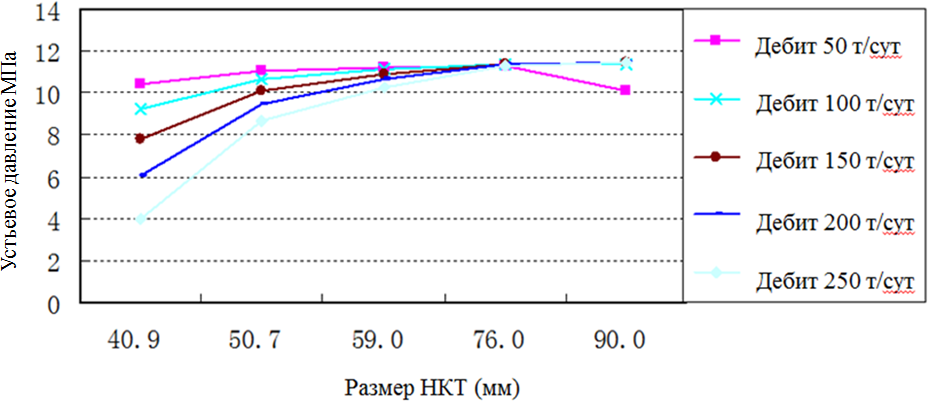
\includegraphics[width=0.7\textwidth]{assets/302}
	\caption*{Рис. 2 - Зависимость устьевого давления от диаметра НКТ (KT-I)}
\end{figure}

\begin{figure}[H]
	\centering
	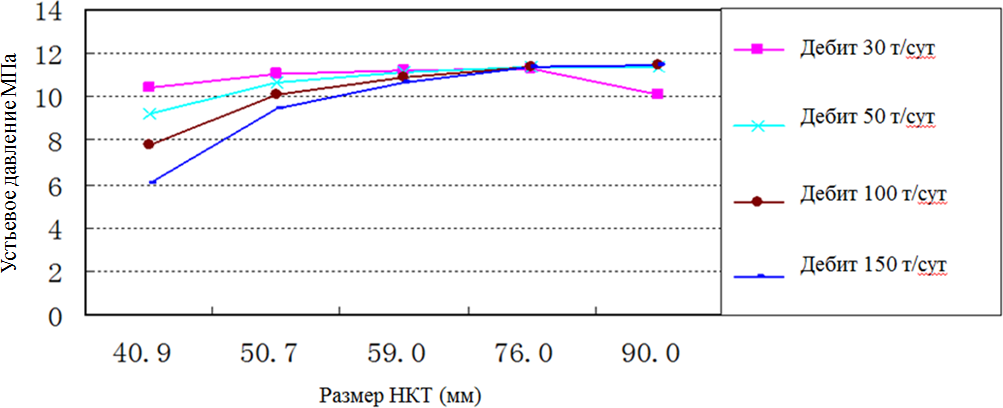
\includegraphics[width=0.7\textwidth]{assets/303}
	\caption*{Рис. 3 - Зависимость устьевого давления от диаметра НКТ (KT-II)}
\end{figure}

\begin{multicols}{2}

Внутрискважинное оборудование фонтанных скважин состоит из
двухступенчатого подъемника, составленного из насосно-компрессорных труб
(НКТ) с наружными диаметрами 73 мм и 88,9 мм, что является рациональным
в условиях эксплуатации месторождения. НКТ Ø89,9 имеет толщину 6,45мм,
Ø73 мм- 7,01 мм.

Для надёжной эксплуатации скважин нефтегазоконденсатного месторождения
исходя из условий эксплуатации, используется следующее подземное
оборудование:

\begin{itemize}
\item
  насосно-компрессорные трубы;
\item
  разобщитель (пакер);
\item
  клапан-отсекатель для автоматического закрытия центрального канала
  скважины;
\item
  башмак колонны НКТ оборудован воронкой в нижней части, которые спущены
  в эксплуатационную колонну диаметром 168,3 и 177,8 мм.
\end{itemize}

Фонтанная арматура скважин соединяется с промысловыми коммуникациями
сбора пластовой жидкости с помощью манифольда, служащего для подключения
к трубному и затрубному пространствам агрегатов для проведения различных
операций при пуске и эксплуатации скважины.

Выбор НКТ Ø89 и Ø73 мм основан на удовлетворении требованиям при КГРП.

В нефтяной залежи KT-I используется комбинированная колонна( Ø89 и Ø73
мм), в которой НКТ Ø89 мм (толщина 6,45 мм) будет иметь длину до 500 м.
В нефтяной залежи KT-IIтакже используется комбинированная колонна, в
которой НКТ Ø89 мм (толщина 6,45 мм), будет длиной 500 м-1000м.

Для обеспечения поддержания высокого устьевого давления при фонтанной
эксплуатации необходим правильный выбор диаметра НКТ. Проведенные
расчеты (Рисунок 2 и 3) определяют использование на месторождении
Северная Трува комбинированных НКТ Ø88,9 мм (толщина 6,45мм) и Ø73 мм
(толщина 7,01мм) {[}14{]}.

{\bfseries Выводы}. На основании расчетов, были определены минимальные давления,
обводненность и другие факторы, при которых скважины прекращают
фонтанирование, что позволяет прогнозировать количество скважин и время
перевода скважин на механизированный способ добычи.

Минимальное устьевое давление прекращения фонтанирования составляет 2
МПа, при этом среднее пластовое давление по I объекту составляет 21 МПа,
среднесуточный дебит скважин -- 100 м\textsuperscript{3}/сут,
обводненность -- 2,8\%, газовый фактор -- 242,8
м\textsuperscript{3}/м\textsuperscript{3}. Согласно проведенным расчетам
в 2021г пластовое давление снизится до 18,8 МПа. Затем панируется рост
пластового давления до 20 МПа, обусловленное влиянием реализации
полномасштабной системы ППД закачкой воды.

По мере повышения объема закачиваемой воды обводненность постепенно
увеличивается, и в 2030г обводненность достигнет 81,2 \%. По прогнозу в
2012г в толще KT-I начнется прекращение фонтанирования, 2023 - 2030гг
являются пиком прекращения фонтанирования, после 2030г основная доля
фонда скважин переводится на механизированный способ эксплуатации.

Среднее пластовое давление по II объекту составляет 29,4 МПа,
среднесуточный дебит скважин -- 48 м\textsuperscript{3}/сут,
обводненность -- 3,9 \%, газовый фактор -- 454
м\textsuperscript{3}/м\textsuperscript{3}. До 2022г согласно выполненным
расчетам пластовое давление будет снижаться до 26,6 МПа, в 2022г, за
счет полномасштабного внедрения системы ППД, наблюдается стабилизация
снижение пластового давления до 2029 года, далее наблюдается тенденция
снижения.

По мере повышения объема закачиваемой воды обводненность продукции
постепенно увеличивается, и в 2030г обводненность продукции достигнет
88,9\%. По прогнозу в 2012г в толще KT-II начнется прекращение
фонтанирования скважин, 2019-2030гг являются пиком прекращения
фонтанирования скважин, после 2030г основная доля фонда скважин
переводится на механизированный способ эксплуатации.
\end{multicols}

\begin{center}
{\bfseries Литература}
\end{center}

\begin{noparindent}
1. В.Н. Бабашев, А.К. Габбасова и др. «Дополнение №1 к проекту оценочных
работ на месторождении Северная Трува»: Отчет, - Алматы: 2015. URL: file:///C:/Users/User/Downloads/PDF\%20(2).pdf

2. Отчет «СНПС Актобемунайгаз», 2023. URL:
http://www.cnpc-amg.kz/?p=senm\_11

3. Групповой технический проект на строительство скважин № 7764, 7804,
829, 538, Н828, 595 месторождения Северная Трува. -Актобе, 2021. URL:

https://www.gov.kz/uploads/2021/12/22/1f923b8735e172674f2771b9b2b72159\_original.1330537.pdf

4.
Джиембаева, К.И., Ахмеджанов Т.К., М. К. Сакиев М.К. Техника и
технология добычи нефти: учебное пособие, - Алматы: Экономика, 2011.
-300 с. ISBN~978-601-225-279-8.

5.
Арбузов В.Н. Эксплуатация нефтяных и газовых скважин. Часть 1: учебное
пособие. -- Томск: ТПУ, 2011. -200 с.

6.
Покрепин Б.В., Гумаров Г.С, Нугманов М.А. Добыча нефти и газа: учебное
пособие. -- Астана: Фолиант, 2011.-392 с. (Профессиональное
образование) ISBN 978-601-292-338-4~

7.
Мищенко И.Т. Скважинная добыча нефти - Москва: Издательский центр РГУ
нефти и газа им. И.М. Губкина, 2015. - 448 с. ISBN 978-5-91961-145-5

8.
Лалазарян Н.В. Эксплуатация нефтяных и газовых скважин. Учебное
пособие. - Алматы: КазНТУ, 2008 -- 140 с. ISBN 978-601-228-026-5

9.
Воцалевский Э.С.,~Даукеев С.Ж.,~Коломиец В.П.,~Комаров
В.П.,~Парагульгов Х.Х.,~Пилифосов В.М.,~Шлыгин Д.А., С.Ж. Даукеев.
Глубинное строение и минеральные ресурсы Казахстана //Нефть и газ.
-Алматы, 2002.- Т. III. -248 с. ISBN 9965-13-760-9.

10.
М.Н. Персиянцев. Добыча нефти в осложненных условиях. -М.:Недра, 2000.
-653 с. ISBN 5-8365-0052-5.

11.
Газизов А.А. Увеличение нефтеотдачи неоднородных пластов на поздней
стадии разпаботки. --М.: ООО Недра-бизнесцентр, 2002. -639 с. ISBN
5-8365-0119-X.

12.
Методические указания по геолого-промысловому анализу разработки
нефтяных и газонефтяных месторождений (РД 153-39.0-110-01).
-Типография "Наука", 121099, Москва,2001.

https://files.stroyinf.ru/Data2/1/4293816/4293816261.pdf

13.
Федорова К.В., Кривова Н.Р, Колесник С.В., Решетникова Д.С. Анализ
состояния выработки запасов нефти из пластов покурской свиты //
Геология, геофизика и разработка нефтяных и газовых месторождений.-
2014. - № 11.- С. 54-58. ISSN 0234-1581

14.
Аржиловский А.В., Гусева Д.Н. Сравнение методов анализ выработки
остаточных запасов // Нефтепромысловое дело. -2016. -№ 10. - С. 14-19.
~ISSN 0207-2351.
\end{noparindent}

\begin{center}
{\bfseries References}
\end{center}

\begin{noparindent}
1. V.N. Babashev, A.K. Gabbasova i dr. «Dopolnenie №1 k proektu
ocenochnyh rabot na mestorozhdenii Severnaja Truva»: Otchet, - Almaty:
2015.

URL: file:///C:/Users/User/Downloads/PDF\%20(2).pdf {[}in Russian{]}

2. Otchet «SNPS Aktobemunajgaz», 2023. URL:
http://www.cnpc-amg.kz/?p=senm\_11 {[}in Russian{]}

3. Gruppovoj tehnicheskij proekt na stroitel\textquotesingle stvo
skvazhin № 7764, 7804, 829, 538, N828, 595 mestorozhdenija Severnaja
Truva. -Aktobe, 2021. URL:

https://www.gov.kz/uploads/2021/12/22/1f923b8735e172674f2771b9b2b72159\_original.1330537.pdf
{[}in Russian{]}

4. Dzhiembaeva, K.I., Ahmedzhanov T.K., M. K. Sakiev M.K. Tehnika i
tehnologija dobychi nefti: uchebnoe posobie, - Almaty: Jekonomika, 2011.
-300 s. ISBN 978-601-225-279-8. {[}in Russian{]}

5. Arbuzov V.N. Jekspluatacija neftjanyh i gazovyh skvazhin.
Chast\textquotesingle{} 1: uchebnoe posobie. -- Tomsk: TPU, 2011. -200
s. {[}in Russian{]}

6. Pokrepin B.V., Gumarov G.S, Nugmanov M.A. Dobycha nefti i gaza:
uchebnoe posobie. -- Astana: Foliant, 2011.-392 s.
(Professional\textquotesingle noe obrazovanie) ISBN 978-601-292-338-4.
{[}in Russian{]}

7. Mishhenko I.T. Skvazhinnaja dobycha nefti - Moskva:
Izdatel\textquotesingle skij centr RGU nefti i gaza im. I.M. Gubkina,
2015. -448 s. ISBN 978-5-91961-145-5. {[}in Russian{]}

8. Lalazarjan N.V. Jekspluatacija neftjanyh i gazovyh skvazhin. Uchebnoe
posobie. - Almaty: KazNTU, 2008 - 140 s. ISBN 978-601-228-026-5. {[}in
Russian{]}

9. Vocalevskij Je.S., Daukeev S.Zh., Kolomiec V.P., Komarov V.P.,
Paragul\textquotesingle gov H.H., Pilifosov V.M., Shlygin D.A., S.Zh.
Daukeev. Glubinnoe stroenie i mineral\textquotesingle nye resursy
Kazahstana //Neft\textquotesingle{} i gaz. -Almaty, 2002.- T. III. -248
s. ISBN: 9965-13-760-9. {[}in Russian{]}

10. M.N. Persijancev. Dobycha nefti v oslozhnennyh uslovijah. -M.:Nedra,
2000. -653 s. ISBN: 5-8365-0052-5. {[}in Russian{]}

11. Gazizov A.A. Uvelichenie nefteotdachi neodnorodnyh plastov na
pozdnej stadii razpabotki. --M.: OOO Nedra-biznescentr, 2002. -639 s.
ISBN 5-8365-0119-X. {[}in Russian{]}

12. Metodicheskie ukazanija po geologo-promyslovomu analizu razrabotki
neftjanyh i gazoneftjanyh

mestorozhdenij (RD 153-39.0-110-01).
-Tipografija "Nauka", 121099, Moskva,2001.

https://files.stroyinf.ru/Data2/1/4293816/4293816261.pdf {[}in
Russian{]}

13. Fedorova K.V., Krivova N.R, Kolesnik S.V., Reshetnikova D.S. Analiz
sostojanija vyrabotki zapasov nefti iz plastov pokurskoj svity //
Geologija, geofizika i razrabotka neftjanyh i gazovyh mestorozhdenij.
-2014.- № 11.- S. 54-58. ISSN 0234-1581 {[}in Russian{]}

14. Arzhilovskij A.V., Guseva D.N. Sravnenie metodov analiz vyrabotki
ostatochnyh zapasov //

Neftepromyslovoe delo. -2016. -№ 10. - S. 14-19.
ISSN 0207-2351. {[}in Russian{]}
\end{noparindent}

{\bfseries \emph{Сведения об авторах}}

\begin{noparindent}
Кайненова Т.С. - магистр, старший преподаватель, Актюбинский
региональный университет им. К.Жубанова, Актобе, Казахстан, е-mail:
kaynenova83@mail.ru;

Космбаева Г.Т. - cтарший преподаватель кафедры «Нефтегазовое дело»
Актюбинского регионального университета им. К. Жубанова, Актобе,
Казахстан, е-mail: gulzhank\_67@mail.ru;

Отарбаева А.Т. - магистр, преподаватель кафедры «Нефтегазовое дело»,
Актюбинский региональный университет им. К. Жубанова, Актобе, Казахстан,
е-mail: ainaerlan1984@mail.ru;

Мерекеқызы А. - cтарший преподаватель кафедры «Нефтегазовое дело»
Актюбинского регионального университета им. К. Жубанова, Актобе,
Казахстан, е-mail: ardak.merekekyzy@mail.ru.

Information about the authors

Kainenova T.S. - Master of Technical Sciences, senior Lecturer, Aktobe
Regional University named after K. Zhubanov, Kazakhstan. е-mail:
kaynenova83@mail.ru;

Kosmbayeva G.T. - Senior Lecturer, Aktobe Regional University named
after K. Zhubanov, Kazakhstan. е-mail: gulzhank\_67@mail.ru;

Otarbayeva A.T. - Master of Technical Sciences, Lecturer, Aktobe
Regional University named after K. Zhubanov, Kazakhstan. е-mail:
ainaerlan1984@mail.ru{\bfseries ;}

Merekeqyzy A. - Senior Lecturer, Aktobe Regional University named after
K. Zhubanov, Kazakhstan. е-mail: ardak.merekekyzy@mail.ru.
\end{noparindent}











